%% BioMed_Central_Tex_Template_v1.06
%%                                      %
%  bmc_article.tex            ver: 1.06 %
%                                       %

%%IMPORTANT: do not delete the first line of this template
%%It must be present to enable the BMC Submission system to
%%recognise this template!!

%%%%%%%%%%%%%%%%%%%%%%%%%%%%%%%%%%%%%%%%%
%%                                     %%
%%  LaTeX template for BioMed Central  %%
%%     journal article submissions     %%
%%                                     %%
%%          <8 June 2012>              %%
%%                                     %%
%%                                     %%
%%%%%%%%%%%%%%%%%%%%%%%%%%%%%%%%%%%%%%%%%


%%%%%%%%%%%%%%%%%%%%%%%%%%%%%%%%%%%%%%%%%%%%%%%%%%%%%%%%%%%%%%%%%%%%%
%%                                                                 %%
%% For instructions on how to fill out this Tex template           %%
%% document please refer to Readme.html and the instructions for   %%
%% authors page on the biomed central website                      %%
%% http://www.biomedcentral.com/info/authors/                      %%
%%                                                                 %%
%% Please do not use \input{...} to include other tex files.       %%
%% Submit your LaTeX manuscript as one .tex document.              %%
%%                                                                 %%
%% All additional figures and files should be attached             %%
%% separately and not embedded in the \TeX\ document itself.       %%
%%                                                                 %%
%% BioMed Central currently use the MikTex distribution of         %%
%% TeX for Windows) of TeX and LaTeX.  This is available from      %%
%% http://www.miktex.org                                           %%
%%                                                                 %%
%%%%%%%%%%%%%%%%%%%%%%%%%%%%%%%%%%%%%%%%%%%%%%%%%%%%%%%%%%%%%%%%%%%%%

%%% additional documentclass options:
%  [doublespacing]
%  [linenumbers]   - put the line numbers on margins

%%% loading packages, author definitions

\documentclass[twocolumn]{bmcart}% uncomment this for twocolumn layout and comment line below
%\documentclass{bmcart}

%%% Load packages
\usepackage{amsthm,amsmath}
%\RequirePackage{natbib}
\RequirePackage[breaklinks=true]{hyperref}
\RequirePackage[authoryear]{natbib}% uncomment this for author-year bibliography
\usepackage[utf8]{inputenc} %unicode support
%\usepackage[applemac]{inputenc} %applemac support if unicode package fails
%\usepackage[latin1]{inputenc} %UNIX support if unicode package fails
\usepackage{graphicx}
\usepackage{listings}
\usepackage{color}
%%%%%%%%%%%%%%%%%%%%%%%%%%%%%%%%%%%%%%%%%%%%%%%%%
%%                                             %%
%%  If you wish to display your graphics for   %%
%%  your own use using includegraphic or       %%
%%  includegraphics, then comment out the      %%
%%  following two lines of code.               %%
%%  NB: These line *must* be included when     %%
%%  submitting to BMC.                         %%
%%  All figure files must be submitted as      %%
%%  separate graphics through the BMC          %%
%%  submission process, not included in the    %%
%%  submitted article.                         %%
%%                                             %%
%%%%%%%%%%%%%%%%%%%%%%%%%%%%%%%%%%%%%%%%%%%%%%%%%


%\def\includegraphic{}
%\def\includegraphics{}

\definecolor{listinggray}{gray}{0.1}
\definecolor{lbcolor}{rgb}{0.9,0.92,0.95}
\lstset{
	backgroundcolor=\color{lbcolor},
	tabsize=4,
	rulecolor=,
	language=Python,
        basicstyle=\scriptsize,
        %upquote=true,
        aboveskip={1.5\baselineskip},
        columns=fixed,
        showstringspaces=false,
        extendedchars=true,
        breaklines=true,
        prebreak = \raisebox{0ex}[0ex][0ex]{\ensuremath{\hookleftarrow}},
        frame=single,
        %showtabs=false,
        %showspaces=false,
        %showstringspaces=false,
        identifierstyle=\ttfamily,
        keywordstyle=\color[rgb]{0,0,1},
        commentstyle=\color[rgb]{0.133,0.545,0.133},
        stringstyle=\color[rgb]{0.627,0.126,0.941},
}

%%% Put your definitions there:
\startlocaldefs
\newcommand{\emma}[1]{{\color{blue}{#1}}}

\endlocaldefs


%%% Begin ...
\begin{document}

%%% Start of article front matter
\begin{frontmatter}

\begin{fmbox}
\dochead{Research}

%%%%%%%%%%%%%%%%%%%%%%%%%%%%%%%%%%%%%%%%%%%%%%
%%                                          %%
%% Enter the title of your article here     %%
%%                                          %%
%%%%%%%%%%%%%%%%%%%%%%%%%%%%%%%%%%%%%%%%%%%%%%

\title{Analyzing microtomography data with Python and the scikit-image
library}

%%%%%%%%%%%%%%%%%%%%%%%%%%%%%%%%%%%%%%%%%%%%%%
%%                                          %%
%% Enter the authors here                   %%
%%                                          %%
%% Specify information, if available,       %%
%% in the form:                             %%
%%   <key>={<id1>,<id2>}                    %%
%%   <key>=                                 %%
%% Comment or delete the keys which are     %%
%% not used. Repeat \author command as much %%
%% as required.                             %%
%%                                          %%
%%%%%%%%%%%%%%%%%%%%%%%%%%%%%%%%%%%%%%%%%%%%%%

\author[
   addressref={aff1},                   % id's of addresses, e.g. {aff1,aff2}
   corref={aff1},                       % id of corresponding address, if any
   %noteref={n1},                        % id's of article notes, if any
   email={emmanuelle.gouillart@nsup.org}   % email address
]{\fnm{Emmanuelle} \snm{Gouillart}}
\author[
   addressref={aff2},
   %email={}
]{\fnm{Juan} \snm{Nunez-Iglesias}}
\author[
   addressref={aff3},
   email={stefanv@berkeley.edu}
]{\fnm{Stéfan} \snm{van der Walt}}



%%%%%%%%%%%%%%%%%%%%%%%%%%%%%%%%%%%%%%%%%%%%%%
%%                                          %%
%% Enter the authors' addresses here        %%
%%                                          %%
%% Repeat \address commands as much as      %%
%% required.                                %%
%%                                          %%
%%%%%%%%%%%%%%%%%%%%%%%%%%%%%%%%%%%%%%%%%%%%%%

\address[id=aff1]{%                           % unique id
  \orgname{Surface du Verre et Interfaces, UMR 125 CNRS/Saint-Gobain}, % university, etc                     %
  \postcode{93303}                                % post or zip code
  \city{Aubervilliers},                              % city
  \cny{France}                                    % country
}
\address[id=aff2]{%
  \orgname{Victorian Life Sciences Computation Initiative, University of Melbourne},
  %\street{700 Swanston St},
  %\postcode{3053}
  \city{Carlton, VIC},
  \cny{Australia}
}
\address[id=aff3]{%
  \orgname{Division of Applied Mathematics, Stellenbosch University},
  %\street{D\"{u}sternbrooker Weg 20},
  %\postcode{24105}
  \city{Stellenbosch},
  \cny{South Africa}
}



%%%%%%%%%%%%%%%%%%%%%%%%%%%%%%%%%%%%%%%%%%%%%%
%%                                          %%
%% Enter short notes here                   %%
%%                                          %%
%% Short notes will be after addresses      %%
%% on first page.                           %%
%%                                          %%
%%%%%%%%%%%%%%%%%%%%%%%%%%%%%%%%%%%%%%%%%%%%%%

%\begin{artnotes}
%\note{Sample of title note}     % note to the article
%\note[id=n1]{Equal contributor} % note, connected to author
%\end{artnotes}

\end{fmbox}% comment this for two column layout

%%%%%%%%%%%%%%%%%%%%%%%%%%%%%%%%%%%%%%%%%%%%%%
%%                                          %%
%% The Abstract begins here                 %%
%%                                          %%
%% Please refer to the Instructions for     %%
%% authors on http://www.biomedcentral.com  %%
%% and include the section headings         %%
%% accordingly for your article type.       %%
%%                                          %%
%%%%%%%%%%%%%%%%%%%%%%%%%%%%%%%%%%%%%%%%%%%%%%

\begin{abstractbox}

\begin{abstract} % abstract
    The exploration and processing of images is a vital aspect of the
    scientific workflows of many X-ray imaging modalities. Users
    require tools that combine interactivity, versatility, and performance.

    \texttt{scikit-image} is an open-source image processing toolkit for
    the Python language that supports a large variety of file formats and
    is compatible with 2-D and 3-D images. The toolkit exposes a simple
    programming interface, with thematic modules grouping functions
    according to their purpose, such as image restoration, segmentation,
    and measurements. \texttt{scikit-image} users benefit from a rich
    scientific Python ecosystem that contains many powerful libraries for
    tasks such as visualization or machine learning.
    \texttt{scikit-image} combines a gentle learning curve, versatile
    image processing capabilities, and the scalable performance required
    for the high-throughput analysis of X-ray imaging data.

\end{abstract}

%%%%%%%%%%%%%%%%%%%%%%%%%%%%%%%%%%%%%%%%%%%%%%
%%                                          %%
%% The keywords begin here                  %%
%%                                          %%
%% Put each keyword in separate \kwd{}.     %%
%%                                          %%
%%%%%%%%%%%%%%%%%%%%%%%%%%%%%%%%%%%%%%%%%%%%%%

\begin{keyword}
\kwd{scikit-image}
\kwd{Python}
\kwd{image processing library}
\kwd{3-D image}
\end{keyword}

% MSC classifications codes, if any
%\begin{keyword}[class=AMS]
%\kwd[Primary ]{}
%\kwd{}
%\kwd[; secondary ]{}
%\end{keyword}

\end{abstractbox}
%
%\end{fmbox}% uncomment this for twcolumn layout

\end{frontmatter}

%%%%%%%%%%%%%%%%%%%%%%%%%%%%%%%%%%%%%%%%%%%%%%
%%                                          %%
%% The Main Body begins here                %%
%%                                          %%
%% Please refer to the instructions for     %%
%% authors on:                              %%
%% http://www.biomedcentral.com/info/authors%%
%% and include the section headings         %%
%% accordingly for your article type.       %%
%%                                          %%
%% See the Results and Discussion section   %%
%% for details on how to create sub-sections%%
%%                                          %%
%% use \cite{...} to cite references        %%
%%  \cite{koon} and                         %%
%%  \cite{oreg,khar,zvai,xjon,schn,pond}    %%
%%  \nocite{smith,marg,hunn,advi,koha,mouse}%%
%%                                          %%
%%%%%%%%%%%%%%%%%%%%%%%%%%%%%%%%%%%%%%%%%%%%%%

%%%%%%%%%%%%%%%%%%%%%%%%% start of article main body
% <put your article body there>

%%%%%%%%%%%%%%%%
%% Background %%
%%
\section*{Introduction}

The acquisition time of synchrotron tomography images has decreased
dramatically over the last decade, from hours to
seconds \citep{Maire2014}. New modalities such as single-bunch
imaging provide a time resolution down to the nanosecond
for radiography \citep{Rack2014}. However, the time subsequently spent in processing the
images has not decreased as much, so that the outcome of a successful
synchrotron imaging run often takes weeks or even months to be
transformed into scientific results. 

Transforming billions of pixels and voxels to a few meaningful figures
represents a tremendous data reduction. Often, the sequence of operations
needed to produce these data is not known beforehand, or might be altered
due to artifacts \citep{Marone2010}, or to an unforeseen evolution of
the sample. Image processing necessarily involves trial and error phases
to choose the processing workflow. Therefore, image processing tools need
to offer at the same time enough flexibility of use, a variety of
algorithms, and efficient implementations to allow for fast iterations
while adjusting the workflow.

Several software applications and libraries are available to synchrotron
users to process their images. ImageJ \citep{Abramoff2004, Schneider2012}
and its distribution Fiji \citep{Schindelin2012} is a popular
general-purpose tool for 2-D and 3-D images, thanks to its intuitive
menus and graphical tools, and the wealth of plugins contributed by a
vivid community \citep{Schindelin2015}. Software specialized in analyzing
synchrotron data are available as well, such as XRDUA~\citep{xrdua} for
diffraction images obtained in powder diffraction analysis, or  For 3-D
images, commercial tools such as Avizo 3D software (TM), or
ToolIP/MAVIkit~\citep{mavi} are appreciated
for an intuitive graphical pipeline and advanced 3D visualization. Some
synchrotrons have even developed their own tools for volume processing,
such as Pore3D~\citep{Brun2010} at the Elettra facility. Alternatively,
the use of a programming language gives finer control, better
reproducibility, and more complex analysis possibilities, provided
classical processing algorithms can be called from libraries -- thereby
limiting the complexity of the programming task and the risk of bugs.
Matlab (TM) and its image processing toolbox are popular in the academic
community of computer vision and image processing. The Python language is
widely used in the scientific world and in synchrotron facilities. As a
general-purpose language, Python is used in synchrotrons to control
device servers \citep{pytango, Sugandhi2016, nsls-ii}, to access raw data
of X-ray detectors \citep{Knudsen2013}, to reconstruct tomography volumes
from radiographs \citep{Gursoy2014, Mirone2014}, and in data processing
packages for macromolecular cristallography \citep{Adams2010}, azimuthal
integration of diffraction data \citep{Ashiotis2015}, or fluorescence
analysis \citep{pymca, Sole2007}. 

%\vskip 1cm 
\texttt{scikit-image}
\citep{Vanderwalt2014} is a general-purpose image processing library for
the Python language, and a component of the ecosystem of Python
scientific modules commonly known as Scientific Python
\citep{Oliphant2007}. Like the rest of the ecosystem,
\texttt{scikit-image} is released under a permissive open-source license
and is available free of charge. Most of \texttt{scikit-image} is
compatible with both 2-D and 3-D images, so that it can be used for a
large number of imaging modalities, such as microscopy, radiography or
tomography. In this article, we explain how \texttt{scikit-image} can be
used for processing data acquired in X-ray imaging experiments, with a
focus on microtomography 3-D images. This article does not intend to be a
pedagogical tutorial on \texttt{scikit-image} for X-ray imaging, but
rather to explain the rationale behind the package, and provide various
examples of its capabilities.


\section*{Methods -- Overview and first steps}

In this section, we provide a short overview of the typical use patterns of
\texttt{scikit-image}, illustrated by short snippets of code. Since
Python is a programming language, the user interacts with data objects and
images through code, which is either entered and executed in an interactive
interpreter, or written in text files (so-called scripts) that are executed. 

\begin{figure*}[!htb]
    \centerline{\includegraphics[width=0.77\textwidth]{ecosystem_landscape}}
    \caption{\csentence{\texttt{scikit-image} and the Scientific Python
	ecosystem}. Images are opened from files as \texttt{NumPy}
	arrays. Functions of \texttt{scikit-image} transform image arrays
	into other arrays with the same dimensions, or into arrays of
	numbers corresponding to features of the image. The output of
	scikit-image functions can be passed to other Python modules
	relying on \texttt{NumPy} arrays, such as \texttt{SciPy} or
	\texttt{scikit-learn}. Image-shaped arrays are transformed into
	visualizations with \texttt{matplotlib} (2D) or \texttt{Mayavi}
	(3D). A variety of environments is available for code development
	and execution, from classical IDEs to Jupyter notebooks.
    \label{fig:ecosystem}}
\end{figure*}


Images are manipulated as numerical arrays, each with a single, uniform
data type.  This common format guarantees interoperability with other
libraries and straightforward access to and interpretation of computer memory. The
N-dimensional (2-D, 3-D, \dots) numerical array object is provided by the
\texttt{NumPy} module \citep{Vanderwalt2011}.

In image processing in Python, one of the first tasks then is to generate
\texttt{NumPy} arrays, which is often achieved by reading data from files. We
read one 2-dimensional image from a file and display it as follows:

\lstinputlisting[language=Python]{io.py} 

\texttt{skimage} is the name under which \texttt{scikit-image} is imported in
Python code. Note that functions (such as \texttt{imread} that reads an image
file, or \texttt{imshow} that displays an image) are found in thematic submodules of
\texttt{skimage}, such as \texttt{io} for Input/Output.

A stack of 2-D images, such as tomography slices generated by a reconstruction algorithm, can be opened as an image collection or a 3-D array:
\lstinputlisting[language=Python]{io_coll.py}
Raw data formats can be opened using the \texttt{NumPy} functions
\texttt{fromfile} (to load the array into memory) or \texttt{memmap} (to
keep the array on disk). The following code creates an array from a
raw image file of unsigned 16-bit integers with a header of 1024 bytes 
\begin{lstlisting}
im = np.memmap('image.edf', shape=(2048, 2048), offset=1024, dtype=np.uint16)
\end{lstlisting}
For every raw data specification, it is thus very easy to write a reader
using \texttt{np.memmap} (see for example
\url{https://github.com/jni/python-redshirt}). 
\texttt{hdf5} files are accessed using modules such as \texttt{h5py}, \texttt{pytables}.
%\texttt{hdf5} files are accessed using modules such as \texttt{h5py}, \texttt{pytables}.

\texttt{scikit-image} has a simple Application Programming Interface
(API), based almost exclusively on
functions. Most functions take an image (\emph{i.e.} a multi-dimensional
array) as input parameter:
\begin{lstlisting}
>>> from skimage import filters
>>> im_gaussian = filters.gaussian(im)
\end{lstlisting}

Optional parameters can be passed as Python \emph{keyword arguments},
in addition to the image parameter.
\begin{lstlisting}
>>> im_gaussian = filters.gaussian(im, sigma=3, mode='wrap')
\end{lstlisting}
A few functions require several arrays to be passed, such as the
watershed segmentation algorithm that takes as parameters the image to be
segmented, and an image of markers from which labels are propagated:
\begin{lstlisting}
>>> from skimage import morphology
>>> labels = morphology.watershed(im, markers)
\end{lstlisting}
Therefore, the image processing workflow can be seen as a directed graph
(a richer structure than a linear pipeline), where nodes are image-shaped arrays, and
edges are functions of \texttt{scikit-image} transforming the arrays (see
Fig.~\ref{fig:ecosystem}).

Most functions transparently handle 2-D, 3-D, or even higher-dimensional
images as arguments, so
the same functions can be used to process tomography, microscopy, or natural
images. The rest raise an error when passed a 3-D argument:
\begin{lstlisting}
>>> filters.prewitt(im)
[...]
ValueError: The parameter `image` must be a 2-dimensional array
\end{lstlisting}
However, the proportion of functions supporting 3D images is always increasing,
thanks to the many contributors to the library.

While the majority of functions return processed images, returns can
also be numerical value(s) such as pixel coordinates of objects of
interest or statistical information about the image:
\begin{lstlisting}
>>> from skimage import exposure
>>> counts, bins = exposure.histogram(im)
>>> counts.shape
(256,)
\end{lstlisting}

\section*{The Python ecosystem}

The benefits of \texttt{scikit-image} for image processing come not only
from the features of the package alone, but also from the rich
environment surrounding scientific Python \citep{Oliphant2007, Perez2011}.
Fig.~\ref{fig:ecosystem} illustrates how several components of this
ecosystem combine into a sophisticated image processing workflow.

\paragraph{NumPy arrays} are the cornerstone of the Scientific Python
ecosystem, and of \texttt{scikit-image} operations in particular.
Cropping or downsampling an image, or retrieving pixels corresponding to
a given label in a segmentation are all NumPy ``one-liners''. To
illustrate the compactness of NumPy code, consider modifying pixel values below a
threshold.  This operation can be written as
\begin{lstlisting}
im[im < 0.5] = 0
\end{lstlisting}
exploiting the ability to index arrays with boolean arrays, also called
\emph{masking}. \texttt{NumPy} uses memory sparingly and avoids
making new copies of arrays whenever possible, an important
requirement when dealing with the gigabyte-sized images of tomography.
For example, cropping a subvolume as follows does not create a copy of the
original array
\begin{lstlisting}
sub_volume = im[100:-100, 100:-100, 100:-100]
\end{lstlisting}
but instead refers to the correct memory offsets in the original.

\paragraph{Interpreter and development environment.}

While several interpreters are available to execute Python instructions
and scripts interactively, the most popular in the scientific world is
IPython \citep{Perez2007, Rossant2015}. IPython is an advanced
interpreter, which integrates syntax highlighting, text auto-completion,
a debugger, introspection and profiling methods, and online help. Several
Integrated Development Environments (IDEs) come bundled with IPython,
together with other components such as a text editor. Notable examples
include Spyder (Fig.~\ref{fig:spyder}), PyCharm, and Visual Studio Code.

\begin{figure*}[!htb]
    \centerline{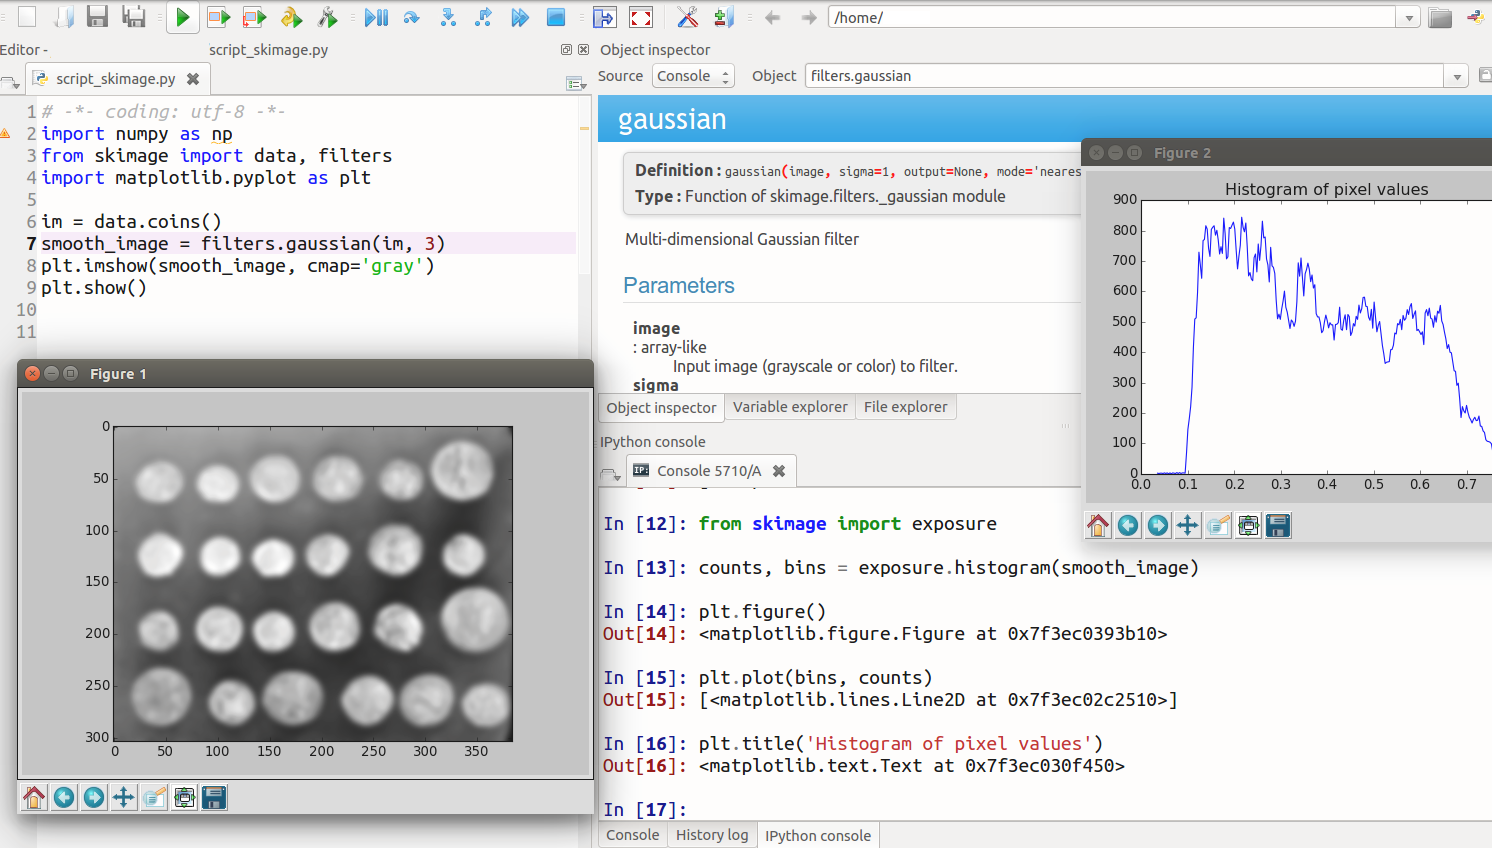
\includegraphics[width=0.99\textwidth]{spyder_process}}
    \caption{\csentence{The Spyder IDE} integrates a text editor (with
	syntax highlighting), the IPython interpreter, as well as a panel
	for code introspection (online help, variable explorer, \dots).
 \label{fig:spyder}}
\end{figure*}

\begin{figure*}[!htb]
    \centerline{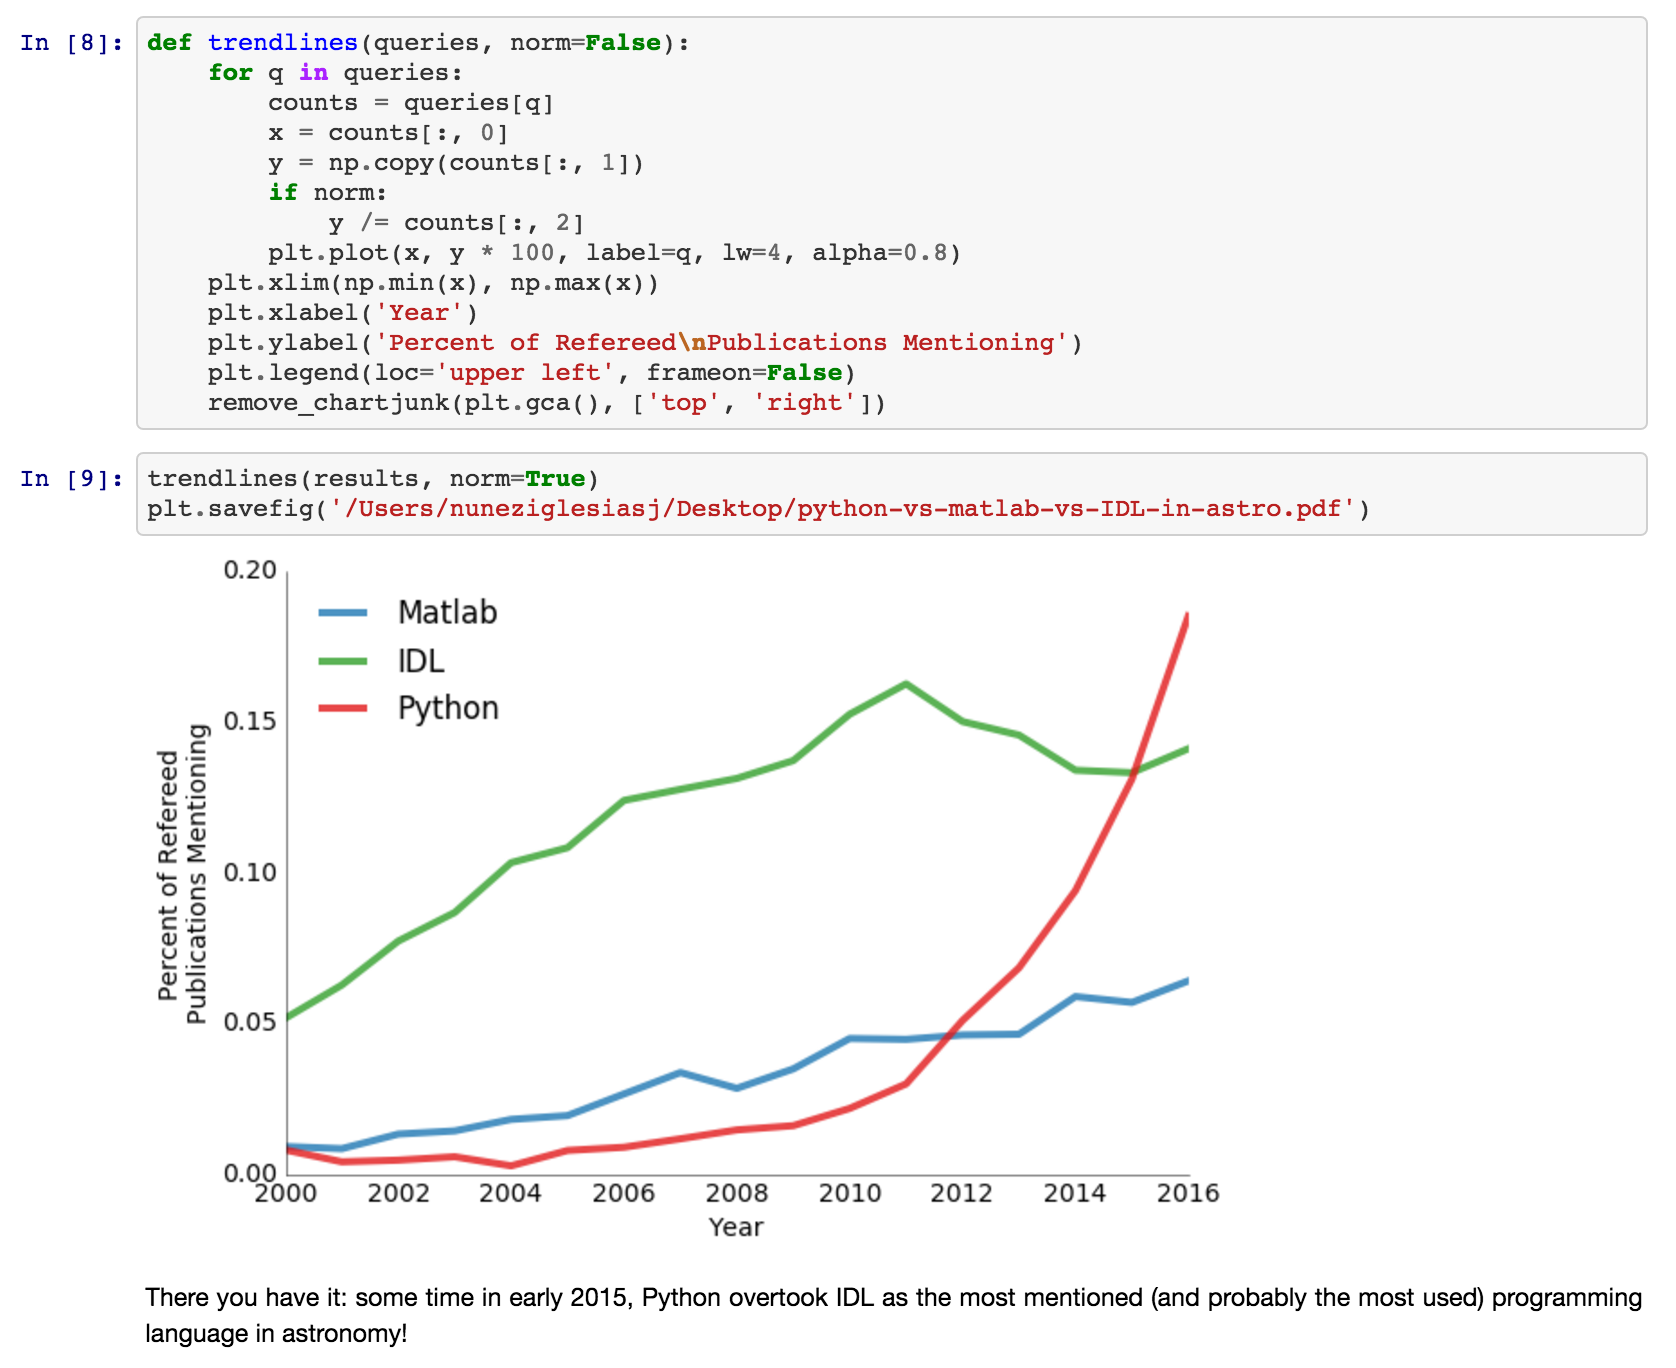
\includegraphics[width=0.75\textwidth]{jupyter_example}}
    \caption{\csentence{The Jupyter notebook} allows mixing of computer code (top),
             plot and text output (middle), and free-form narrative text (bottom).
             This makes it ideal to record and report code-based analyses.
             Screenshot from \cite{NunezIglesias2016}.
 \label{fig:jupyter}}
\end{figure*}

The Jupyter notebook \citep{Kluyver2016} is a web application that grew
out of the IPython project. Jupyter notebooks provide an interactive
development environment within a web browser, where live code can be
enriched by explanatory text, equations and visualizations
(Fig.~\ref{fig:jupyter}). Jupyter notebooks render directly as webpages
on GitHub, making them a straightforward tool to publish online a
script and its output. As of July 2016, more than 500,000 Jupyter
notebooks were posted on GitHub, demonstrating their wide adoption by the
community as workflow-sharing tools
(\url{http://archive.ipython.org/media/SciPy2016JupyterLab.pdf}).


\paragraph{Visualization libraries.}


Visualizing images is an important component of the image processing
workflow, used to inspect the final result and to adjust the
parameters of intermediate processing operations.
\texttt{matplotlib} \citep{Hunter2007} is the most popular 2D plotting
library of the Python ecosystem. It can be used to visualize 2D data such
as color or grayscale images, and 1D data such as contour lines, outlines
of segmented regions, histograms of gray levels, etc. Although
\texttt{matplotlib} has simple 3D plotting capabilities, we
recommend using the \texttt{mayavi} module \citep{Ramachandran2011}
for applications requiring advanced 3D visualization, such as tomography. 
\texttt{mayavi} is based on the VTK toolkit. It exposes a simple API for
visualizing data passed as \texttt{numpy} arrays. For example,
visualizing the surface of binary data can be written as
\begin{lstlisting}[language=Python]
# synthetic binary array from skimage.data
im = data.binary_blobs(length=400, n_dim=3).astype(np.uint8)
# visualization
from mayavi import mlab
mlab.contour3d(im)
mlab.outline()
\end{lstlisting}
(see Fig.~\ref{fig:mayavi} for the resulting visualization).

For more advanced visualizations, a large majority of VTK capabilities
can be accessed through mayavi's pipeline API. \texttt{mayavi} offers a
good trade-off between simplicity of use for common operations, and
accessibility to more sophisticated capabilities such as responsive
visualizations.


\paragraph{Advanced toolkits for signal processing and data science.}

\texttt{scikit-image} is only one Python module that can be used for data
processing, among many others. A very popular module is
\texttt{scikit-learn} \citep{Pedregosa2011}, a Python module for machine
learning using \texttt{NumPy} arrays. Local features of an image
(such as local statistics of gray levels, or geometric points of
interest) or features of segmented objects (e.g. geometrical and
intensity characteristics of segmented particles) can be extracted with
functions from \texttt{skimage.feature} (see Fig.~\ref{fig:ecosystem}). It
is then possible to use a \emph{classification} algorithm from
\texttt{scikit-learn} to label pixels (a segmentation task)
or to classify whole images or objects that have already been segmented.
The near-universal use of \texttt{NumPy} arrays ensures the interoperability
between these packages, so that just a few lines of code are sufficient
to create these sophisticated workflows.

The modularity of the Scientific Python ecosystem may be
confusing at first sight, but the core modules of this ecosystem
are almost perfectly compatible, thanks to the shared use of NumPy arrays
and common development practices (although they are developed in parallel
by different teams). Several ``distributions'', such as Anaconda
or Canopy, bundle together the most popular libraries, including
\texttt{scikit-image}.

\section*{Results}
\begin{figure}[!htb]
    \centerline{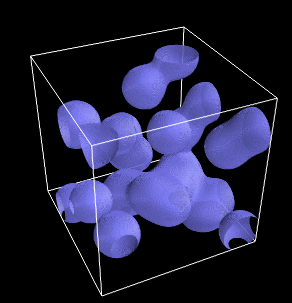
\includegraphics[width=0.6\columnwidth]{mayavi_example}}
    \caption{\csentence{Simple 3-D visualization} realized with Mayavi.
 \label{fig:mayavi}}
\end{figure}



\section*{Image processing capabilities}

\begin{figure*}
    \centerline{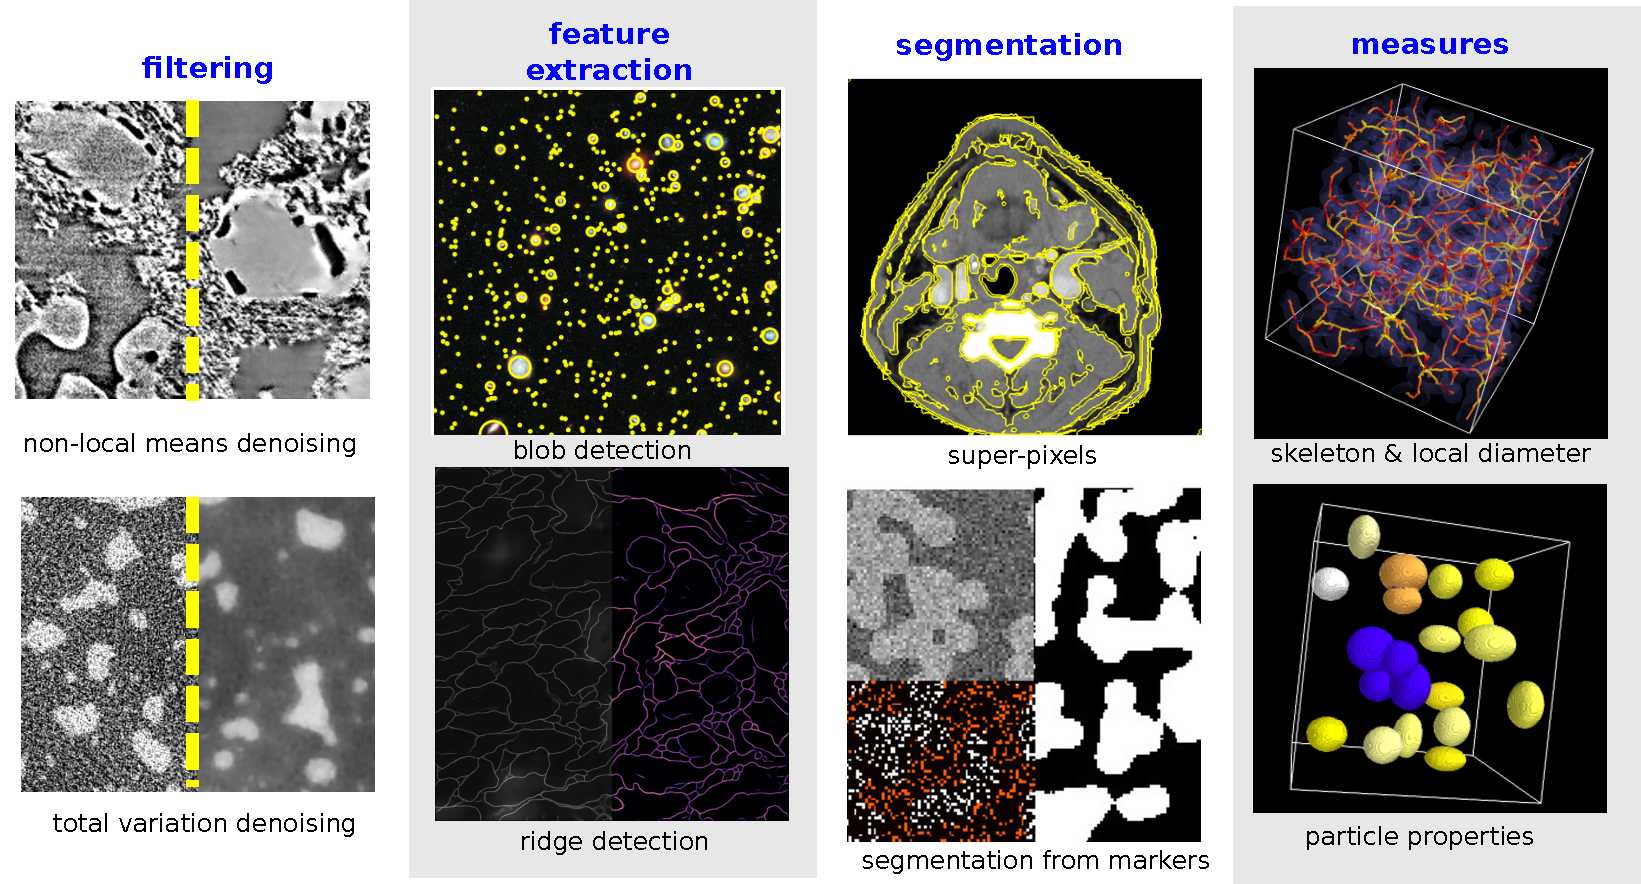
\includegraphics[width=0.99\textwidth]{tomo_gallery}}
    \caption{\csentence{Typical image processing operations with
	\texttt{scikit-image}.}
	Data are synthetic, unless stated otherwise.
	\textbf{a) Filtering -} Top: non-local means denoising of an image
	with a fine-grained texture, acquired by \emph{in situ}
	synchrotron microtomography during
	glass melting \citep{Gouillart2012}. Bottom: total-variation
	denoising of an image with two phases, corresponding to
	phase-separating silicate melts observed by \emph{in situ
	tomography} \citep{Bouttes2015}.
	\textbf{b) Feature extraction -} Top: Hubble deep field (NASA,
	public domain), blob detection using the
	Laplacian of Gaussian method. Bottom: ridge detection using the
	leading eigenvalue of the Hessian matrix, neuron image from
	CREMI challenge (\url{https://cremi.org/data/}).
	\textbf{c) Segmentation - } Top: super-pixel segmentation
	of a CT slice of the human head \citep{tomo_wikipedia}, using
	Felzenszwalb's algorithm \citep{Felzenszwalb2004}. Bottom: random
	walker segmentation (right) of noisy image (top-left corner), using
	histogram-determined markers (bottom-left corner).
	\textbf{d) Measures -} Top: visualization of local diameter
	(color-coded on the skeleton curve) of an
	interconnected phase (represented in violet).  Bottom: particles color-coded according
	to their extent.
\label{fig:tomo_gallery}}
\end{figure*}

\paragraph{Capabilities.}

\texttt{scikit-image} offers most classical image processing operations,
such as exposure and color adjustment, filtering, segmentation, feature
extraction, geometric transformations, and measurements of region
characteristics. In addition to common operations, some advanced
algorithms are also implemented, a selection of which is illustrated in
Fig.~\ref{fig:tomo_gallery}. In the following, we briefly illustrate how
\texttt{scikit-image} can be used for some typical image processing
tasks encountered when analyzing tomographic images: denoising, mid-range
feature detection, segmentation and measurement of region properties. For
the sake of brevity, other tasks such as contrast manipulation or
geometric transformations are not described here; the interested reader
is referred to the documentation of \texttt{scikit-image}.

Tomographic images often suffer from artifacts or poor signal-to-noise
ratio. Therefore, \emph{denoising} data is often the first step of an
image processing workflow. Several denoising filters are available for
restoring these images, ranging from general-purpose median and
bilateral filters to those more suited to specific applications. For
example, total-variation denoising \citep{Chambolle2004, Getreuer2012} is
ideal for restoring piecewise-constant images (see
Fig.~\ref{fig:tomo_gallery} a)), such as images with a small number of
phases encountered in materials science \citep{Bouttes2015}. Conversely,
images with a fine-grained texture are better preserved with non-local
means denoising, a patch-based algorithm \citep{Buades2005} (see
Fig.~\ref{fig:tomo_gallery} a)). 

Detecting the presence of objects or extracting pixels corresponding to
objects (a task known as segmentation) is an important task of image
analysis for medical or materials science applications.
\texttt{scikit-image} offers a wide variety of functions for
\emph{detecting geometrical features} of interest in an image. In order
to detect thin boundaries, the ridges of an image can be identified as
regions for which the leading eigenvalue of the local Hessian matrix is
high (see Fig.~\ref{fig:tomo_gallery} b)). In the Fourier space, peaks in
2D Bragg diffraction patterns can be extracted using blob detection
methods \citep{Ashiotis2015}, such as the Laplacian of Gaussian method
(see Fig.~\ref{fig:tomo_gallery} b)). 

\emph{Segmentation} of regions of interest can be achieved using one of various
strategies, depending on the characteristics of the image. Images with a
clear contrast between regions can be segmented automatically thanks to
several thresholding algorithms, including an adaptive local thresholding
algorithm aimed at images with contrast variations. Super-pixel
algorithms \citep{Felzenszwalb2004, Achanta2012} create an
over-segmentation of images in super-pixels, by grouping pixels that are
close together both in color- and spatial distance (see
Fig.~\ref{fig:tomo_gallery} c)). Region-growing algorithms, such as the
morphological watershed or the random walker \citep{Grady2006}, propagate
the labels of user-defined markers through the image (see
Fig.~\ref{fig:tomo_gallery} c)). The active contour algorithm
\citep{Kass1988} fits snake contours to features of the image, such as
edges or high-brightness regions.

Following segmentation, the characteristics of labeled regions
(particles, porosities, organs, \dots) resulting from a segmentation can
be measured using the \texttt{measure} submodule. The different connected
components (e.g. bubbles or non-touching particles) of a binary image are
labeled with the \texttt{measure.label} function. Properties of labeled
regions such as size, extent, center of mass or mean intensity value are
accessed with \texttt{measure.regionprops} (see
Fig.~\ref{fig:tomo_gallery} d)). Local characteristics of a region can be
retrieved as well: Fig.~\ref{fig:tomo_gallery} d) shows how the local
diameter of open porosity is measured by combining a skeletonization of
the porosity channels, and the distance transform to the other phase
measured on the skeleton.   

\paragraph{Performance.}

Given the large size of tomography datasets, the execution speed of image
processing operations is of critical concern. \texttt{scikit-image}
relies mostly on calls to \texttt{NumPy} operations, of which most are
performed in optimized compiled code (C or Fortran). Performance-critical
parts of \texttt{scikit-image} that cannot call efficient \texttt{NumPy}
code are implemented in \texttt{Cython}. \texttt{Cython}
\citep{Behnel2011} is an extension of the Python language that supports
explicit type declarations, and is compiled directly to C. Therefore, the
performance of \texttt{scikit-image} can be close to the one of libraries
written in a compiled language such as C++ or Java. For example,
computing the watershed segmentation of a 2000x2000 array of floats into
1000 regions took about 1 s using 1 CPU of an off-the-shelf laptop, and
10 s for a 256x256x256 image segmented into 2000 regions. Similar
timescales were obtained with \texttt{mahotas}, a Python package
implemented exclusively in C++ \citep{Coelho2013} (with a slight advantage
for \texttt{mahotas}).

However, basic \texttt{scikit-image} code runs on a single core. Computing
workstations and servers used for X-ray imaging typically have several tens of
cores. Parallelization of the computing workflow can be achieved in multiple
ways. The most trivial parallelization scheme consists of applying the same
workflow to different images, on different cores. However, finer-grained
parallelization is preferable when prototyping the processing workflow.


An easy solution consists in dividing an image into smaller images (with
or without overlap, depending on the operation), and to apply the
same operation on the different sub-images, on different cores. Creating overlapping chunks is easy with the dedicated function \texttt{view\_as\_windows} (or \texttt{view\_as\_blocks} for contiguous non-overlapping chunks):
\begin{lstlisting}[language=Python]
>>> from skimage import util, data
>>> im = data.camera()
>>> im.shape
(512, 512)
>>> # chunks of size 134 with 8-pixel overlap
>>> chunks = util.view_as_windows(im, (134, 134), step=126)
>>> chunks.shape
(4, 4, 134, 134)
\end{lstlisting}
The \texttt{joblib} library enables easy parallel processing. Looping over the different blocks, and dispatching the computation over several cores, is realized with the following syntax:
\begin{lstlisting}
>>> from joblib import Parallel, delayed
>>> filtered_chunks = Parallel(n_jobs=4)(delayed(filters.gaussian)(chunks[i, j]) for i in range(4) for j in range(4))
\end{lstlisting}
\texttt{scikit-image} also offers experimental support for a more integrated parallel processing pipeline, thanks to the \texttt{dask} \citep{dask} module:
\begin{lstlisting}
filtered_im = util.apply_parallel(filters.gaussian, im, depth=8)
\end{lstlisting}
The size of chunks is determined automatically from the number of available cpus, or can be specified by the user.

{\em Caching} provides another tool to speed up data analysis. A situation
that often arises is that, while prototyping a workflow, scripts
(containing the image processing pipeline) are run several times to
experiment with parameters. \texttt{joblib} provides a caching mechanism
that avoids the repetition of function calls, if their arguments have not
changed:
\begin{lstlisting}
>>> from skimage import filters, data
>>> from joblib import Memory
>>> mem = Memory(cachedir='/tmp/joblib')
>>> median = mem.cache(filters.median)
>>> im = data.camera()
>>> filtered_im = median(im, np.ones((3, 3)))
__________________________
[Memory] Calling skimage.filters.rank.generic.median...
median(array([[156, ..., 152],
       ..., 
       [121, ..., 111]], dtype=uint8), array([[ 1.,  1.,  1.],
       [ 1.,  1.,  1.],
       [ 1.,  1.,  1.]]))
__________________________median - 0.0s, 0.0min
>>> filtered_again = median(im, np.ones((3, 3)))
>>> # the above call did not trigger another evaluation
\end{lstlisting}

Finally, we note that the biggest performance improvements often come from
the improvement of algorithms (as opposed to computing architectures only). For
example, non-local means denoising \citep{Buades2005} is a costly operation,
since it requires several nested loops, on all pixels and on neighboring
patches to be compared with the pixel-centered patch. Thanks to the
implementation of a more recent algorithm \citep{Darbon2008} that modifies the
internal organization of loops, it was possible to improve execution
time by a factor of roughly ten times.
The large size of the \texttt{scikit-image} community makes it likely for
algorithmic improvements to be discussed regularly. During the code review
process, a close watch is also kept on memory consumption, since for
large image sizes, transfers between computer memory (RAM) and CPU cache
are often a serious performance bottleneck.



\section*{Documentation}

The quality of software documentation is (perhaps especially) important
in software aimed at scientists. \texttt{scikit-image} users have access
to several kinds of documentation. All functions are documented using the
NumPy documentation standard \citep{Pawlik2015}, which is universal
across all major Scientific Python packages. The standard include a
description of all input and output variables and their data types,
together with explanations of what each function does and how to use it.
Function documentation is accessible online or within the development
environment itself (IPython, Spyder, Jupyter Notebook...).

\begin{figure*}
    \centerline{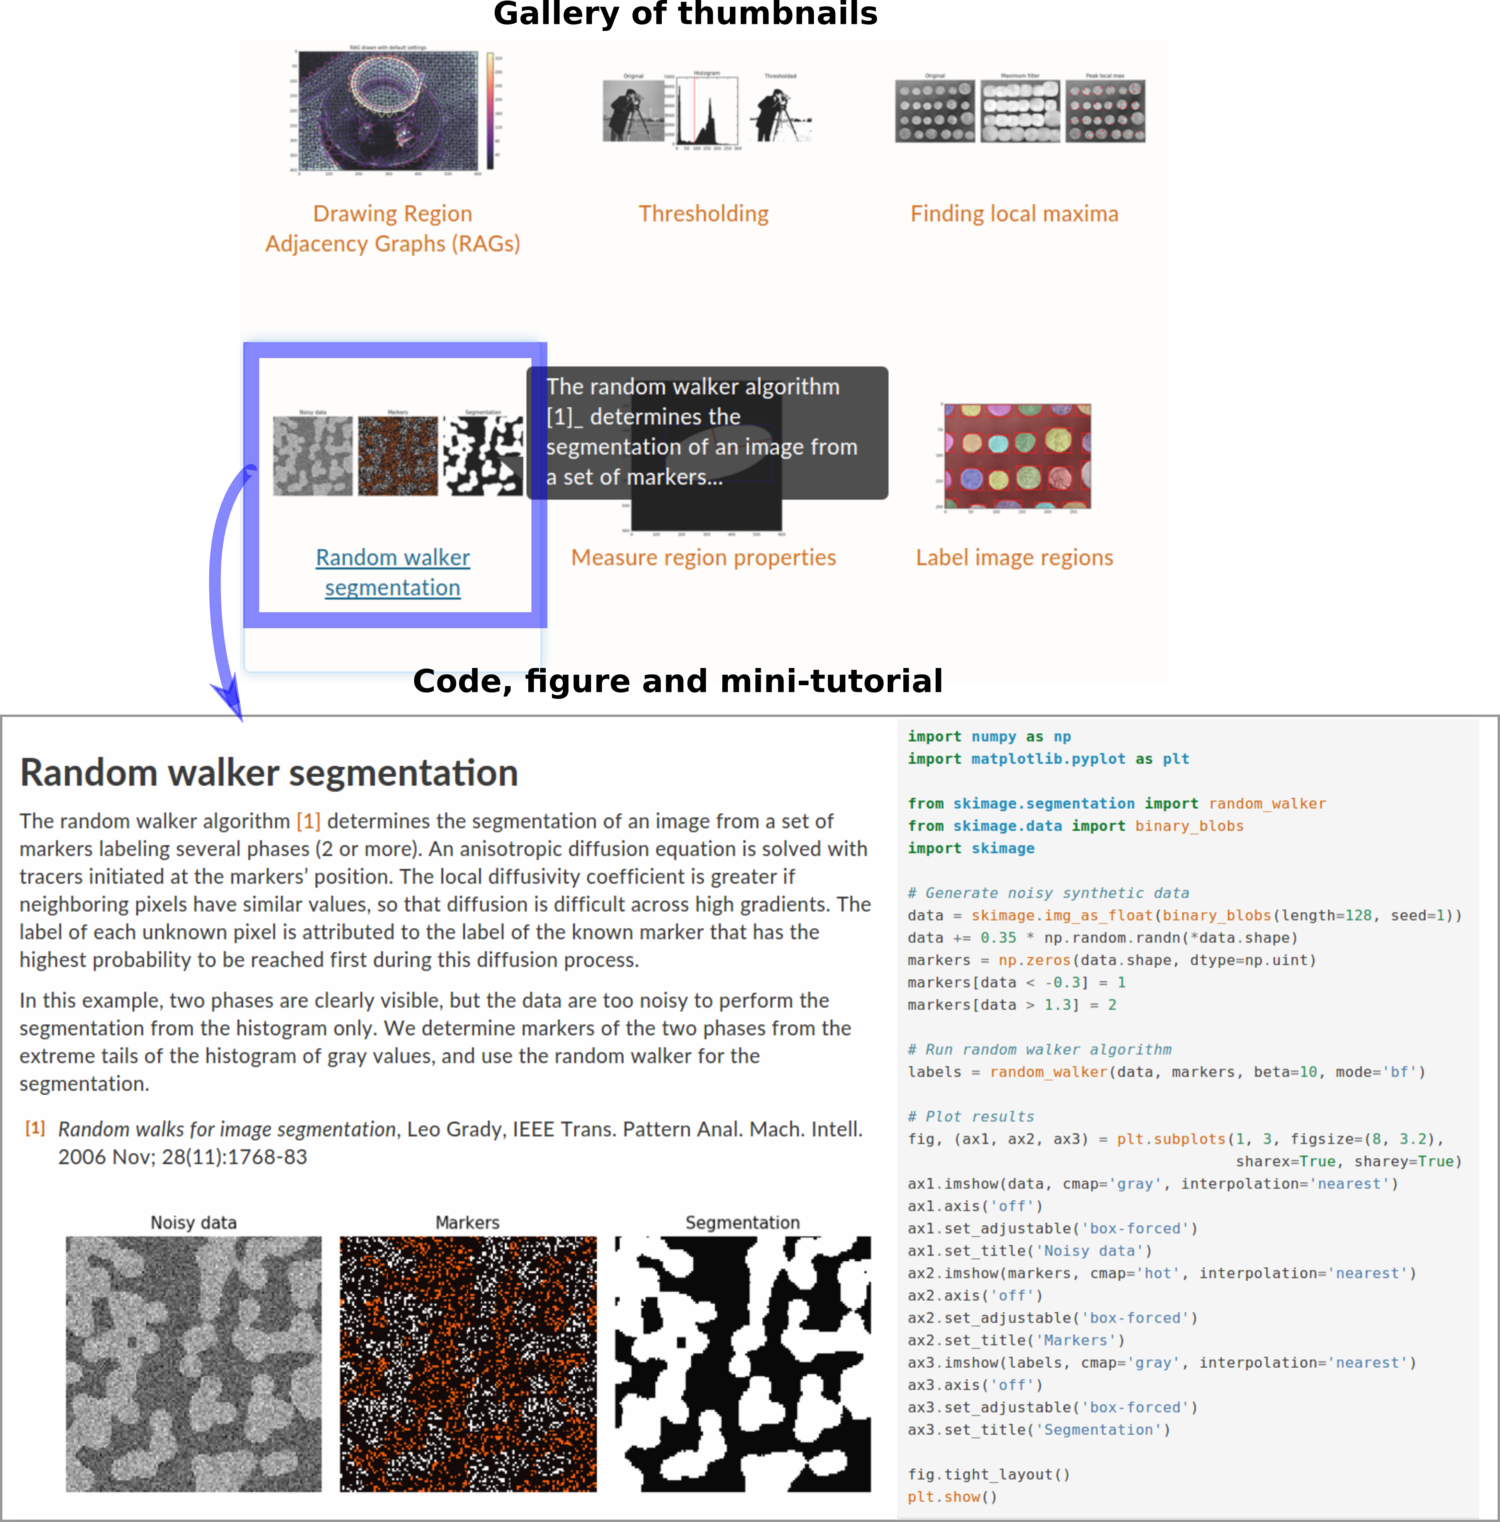
\includegraphics[width=0.95\textwidth]{figure_gallery}}
\caption{\csentence{Gallery of examples of \texttt{scikit-image}.}
 The gallery of examples consists of an array of thumbnails (left), which link to example webpages, each centered on a specific image processing task. Each webpage includes Python code generating a figure, the figure itself, and a short tutorial explaining the image processing operations and the code. \label{fig:gallery}}
\end{figure*}

In addition, a graphical gallery of examples
(\nolinkurl{http://scikit-image.org/docs/dev/auto_examples/}), part of
which is displayed in Fig.~\ref{fig:gallery}, showcases graphical
examples of common image processing operations.  The examples are
organized as an array of thumbnails with a short title (see
Fig.~\ref{fig:gallery} left). These thumbnails link to the webpage of the
corresponding example, which features a mini-tutorial on the image
processing method, the code needed to run the example and the figure
generated by the example. Since the graphical gallery is an efficient way
to inform users about the features of \texttt{scikit-image}, every new
feature integrated in the package must include an example for the
gallery. Longer tutorials and a more narrative documentation is available
as well in the online User Guide of \texttt{scikit-image}. The User Guide
explains in particular "big picture", foundational aspects of
\texttt{scikit-image}, such as its use of \texttt{NumPy} arrays as
images, or how the package interacts with other parts of the scientific
Python ecosystem.

Finally, tutorials on \texttt{scikit-image} are available in various
places, either as YouTube videos, or in the SciPy Lecture
Notes \citep{scipylecturenotes}, a comprehensive online book of Scientific
Python tutorials.  

\section*{Development and use of scikit-image}

\paragraph{Who uses scikit-image.}

Estimating the number of active users of an open-source package is a
difficult task. Download statistics, for example, largely
overestimate the number of active users, all the more if the package is
bundled with others in a software distribution, such as Anaconda or
Canopy. A view closer to reality can be obtained by analyzing the
statistics of visits of the online help, available on the project
website.  As of the first half of 2016, 20000 unique visitors visited the
\texttt{scikit-image} website every month at
\url{http://scikit-image.org/}, from 138 countries.

The \texttt{scikit-image} paper of 2014 \citep{Vanderwalt2014} has been
cited by 120 research works (as of August 2016, according to Google
Scholar), among which studies that used X-ray imaging in fields such as
medical imaging \citep{Shen2015, Malan2016, Blackledge2016}, materials
science \citep{Bouttes2015} or geoscience \citep{Schluter2014}.

\paragraph{Development process.}

\texttt{scikit-image} is developed by a diverse team of volunteers.
More than 170 individuals have contributed to the package. The large
number of developers and users key to project's sustainability. The
development process takes place on GitHub
\url{https://github.com/scikit-image/scikit-image}, where users and
developers propose and discuss new contributions, report bugs or submit ideas
for improvements.
A release cycle of one or two releases every year
ensures that new features are propagated to users on a regular basis.

\section*{Discussion -- Current limitations and challenges}

While we emphasize the assets of \texttt{scikit-image} for processing
X-ray images, one should be aware of current limitations.

\paragraph{Speed of execution.} Although \texttt{scikit-image} approaches
the speed of execution of compiled (C++, Java) code, it cannot reach the
performance of code optimized for the GPU, or the hand-tuned
CPU-specific optimizations found in OpenCV \citep{Pulli2012}. At the moment,
\texttt{scikit-image} is not the best tool for ultrafast computations
where the workflow is known beforehand, simple and stable. However, it is
an excellent tool for exploring image data interactively and testing
different algorithms -- an important component of data processing in
scientific work --, and its speed of execution is sufficient for processing
gigabyte-sized tomographic images in seconds to minutes. Moreover,
the multiprocessing capability of \texttt{scikit-image} is likely to improve in
the near future.

\paragraph{3-D compatibility.} Currently, about two thirds of
\texttt{scikit-image} functions transparently handle 2D or 3D arrays, with
the remainder limited to 2D analysis, often unnecessarily. Improved support
for 3D and higher-dimensional volumes is on the project roadmap.

\paragraph{Documentation for domain-specific applications.} Some image
processing libraries or applications address a specific scientific
domain, such as CellProfiler \citep{Carpenter2006, Lamprecht2007} for
biological images. The documentation of such projects often showcases
examples that are close to the experience of the targeted community.
Since \texttt{scikit-image} is application-agnostic,
applications such as tomographic imaging are not mentioned in detail in the
documentation of \texttt{scikit-image}. A possible improvement would be
to write comprehensive tutorials addressing specific communities, and to
refer to these tutorials from the main \texttt{scikit-image}
documentation.

\section*{Getting started}

Scientists interested in experimenting with \texttt{scikit-image} are
invited to read the installation instructions at
\url{http://scikit-image.org/docs/stable/install.html}.
\texttt{scikit-image} can be installed either bundled in a Scientific
Python distribution, such as Anaconda (conda command line) or Canopy, or
stand alone (along with its dependencies) using a installer/packager such
as pip or Ubuntu's Aptitude.

The Getting Started section of the online User Guide
(\url{http://scikit-image.org/docs/dev/user_guide/getting_started.html})
provides a good launch pad for beginners, and gently leads into other sections of the user
guide. A gallery of examples
(\url{http://scikit-image.org/docs/dev/auto_examples/}) lets users
find applications close to their needs. Although most examples in the
gallery use 2D images, many are applicable to 3D images as well.

Assistance on matters not covered by the documentation is provided on
the dedicated mailing-list \url{scikit-image@googlegroups.com} or on
StackOverflow
\url{http://stackoverflow.com/questions/tagged/scikit-image}.

\section*{Conclusion}

\texttt{scikit-image} offers a wide variety of image processing
algorithms, using a simple interface natively compatible with 2D and 3D
images. It is well integrated into the Scientific Python ecosystem, so
that it interfaces well with visualization libraries and other data
processing packages. \texttt{scikit-image} has seen tremendous growth
since its creation in 2009, both in terms of users and included features.
In addition to the growing number of scientific teams that use
\texttt{scikit-image} for processing images of various X-ray modalities,
domain-specific tools are now using \texttt{scikit-image} as a dependency
to build upon. Examples include \texttt{tomopy} \citep{Gursoy2014} for
tomographic reconstruction, or \texttt{DIOPTAS} \citep{Prescher2015} for
the reduction and exploration of X-ray diffraction data. It is likely
that more application-specific software will benefit from depending on
\texttt{scikit-image} in the future, since \texttt{scikit-image} strives
to be domain-agnostic and to keep the function interface stable. On the end-user
side, future work includes better integration of parallel processing
capabilities, completion of full 3-D compatibility, an enriched narrative
documentation, speed enhancements, and expansion of the set of supported algorithms.

%%%%%%%%%%%%%%%%%%%%%%%%%%%%%%%%%%%%%%%%%%%%%%
%%                                          %%
%% Backmatter begins here                   %%
%%                                          %%
%%%%%%%%%%%%%%%%%%%%%%%%%%%%%%%%%%%%%%%%%%%%%%

\begin{backmatter}

\section*{Competing interests}
The authors declare that the research was conducted
in the absence of any commercial or financial relationships that could be
construed as a potential conflict of interest.

\section*{Author's contributions}
E. Gouillart, J. Nunez Iglesias and S. van der Walt conducted the
research and wrote the paper. All authors read and approved the final
manuscript.


\section*{Acknowledgements}
  
The authors gratefully acknowledge the work of the contributors of
  \texttt{scikit-image}, and thank S. Deville and D. Vandembroucq for a
  careful reading of the paper and useful suggestions. E. Gouillart
  acknowledges the support of ANR project EDDAM ANR-11-BS09-027. CREMI
  (https://cremi.org/data/) is acknowledged for the membrane image of
  Fig.~\ref{fig:tomo_gallery} (b). 

%%%%%%%%%%%%%%%%%%%%%%%%%%%%%%%%%%%%%%%%%%%%%%%%%%%%%%%%%%%%%
%%                  The Bibliography                       %%
%%                                                         %%
%%  Bmc_mathpys.bst  will be used to                       %%
%%  create a .BBL file for submission.                     %%
%%  After submission of the .TEX file,                     %%
%%  you will be prompted to submit your .BBL file.         %%
%%                                                         %%
%%                                                         %%
%%  Note that the displayed Bibliography will not          %%
%%  necessarily be rendered by Latex exactly as specified  %%
%%  in the online Instructions for Authors.                %%
%%                                                         %%
%%%%%%%%%%%%%%%%%%%%%%%%%%%%%%%%%%%%%%%%%%%%%%%%%%%%%%%%%%%%%

% if your bibliography is in bibtex format, use those commands:
\bibliographystyle{bmc-mathphys} % Style BST file (bmc-mathphys, vancouver, spbasic).
\bibliography{refs}      % Bibliography file (usually '*.bib' )
% for author-year bibliography (bmc-mathphys or spbasic)
% a) write to bib file (bmc-mathphys only)
% @settings{label, options="nameyear"}
% b) uncomment next line
\nocite{label}

% or include bibliography directly:
% \begin{thebibliography}
% \bibitem{b1}
% \end{thebibliography}

\newpage
~
\newpage

\section*{Figures}

\listoffigures

%%%%%%%%%%%%%%%%%%%%%%%%%%%%%%%%%%%
%%                               %%
%% Figures                       %%
%%                               %%
%% NB: this is for captions and  %%
%% Titles. All graphics must be  %%
%% submitted separately and NOT  %%
%% included in the Tex document  %%
%%                               %%
%%%%%%%%%%%%%%%%%%%%%%%%%%%%%%%%%%%

%%
%% Do not use \listoffigures as most will included as separate files

%%%%%%%%%%%%%%%%%%%%%%%%%%%%%%%%%%%
%%                               %%
%% Tables                        %%
%%                               %%
%%%%%%%%%%%%%%%%%%%%%%%%%%%%%%%%%%%

%% Use of \listoftables is discouraged.
%%
%%%%%%%%%%%%%%%%%%%%%%%%%%%%%%%%%%%
%%                               %%
%% Additional Files              %%
%%                               %%
%%%%%%%%%%%%%%%%%%%%%%%%%%%%%%%%%%%



\end{backmatter}
\end{document}
